\documentclass{scrreprt}
\usepackage[utf8]{inputenc}
\usepackage[ngerman]{babel}
\usepackage{pslatex}
%%\setkomafont{sectioning}{\bfseries}
%%\usepackage{amsmath}
%%\usepackage[a4paper, left=4cm, right=2.0cm, top=2cm, bottom=2cm]{geometry}
%%\usepackage{scrpage2}
%%\clearscrheadfoot
%%\chead[-\pagemark-]{-\pagemark-} 
%%\pagestyle{scrheadings}
\usepackage{lipsum}
\linespread {1.5}
\usepackage{hyperref}
%%\usepackage{textcomp}
\usepackage{graphicx}

 
\title{W.O.R.M.}
\author{Wreck Opponents Repeatedly Meaningless}
\begin{document}
 
\maketitle
\tableofcontents
\thispagestyle{empty}
\newpage
\setcounter{page}{3}

\chapter{Einführung}
Die Ideen und die Art und Weise des Spieles W.O.R.M. wurde aus der Spielreihe der Worms\-spiele
entnommen. Worms selber ist eine Serie von taktischen rundenbasierten Multiplayer-Computerspielen,
die auch bei W.O.R.M. beibehalten wurde. Bei  W.O.R.M. können bis zwei bis vier Spieler
mitspielen.

Jeder Spieler erhält ein Team von drei Würmern und sucht vor dem Spiel seine Waffen aus, die
er dann unterschiedlich im Spiel benutzen kann. Beim Treffen eines Wurms, sei es der Gegner
oder der eigene Wurm, verringert sich das Leben, das über den Würmern in der vorher
ausgewählten Teamfarbe erscheint. Haben die Würmer keine Lebenspunkte mehr sterben sie und
können nicht mehr benutzt werden. Das Spiel endet wenn ein Team keine Würmer mehr
hat.

Jeder Spieler hat im Spiel 20 Sekunden Zeit seinen Wurm in alle Richtungen zu Bewegen. Die
Runde ist vorbei wenn der Wurm mit seiner Waffe geschossen hat oder wenn die 20 Sekunden
zu Ende sind. Zu Beginn es Spiels erscheinen Items an verschiedenen Positionen, die den Würmern
im Spiel extra Fähigkeiten bieten (siehe im Benutzerhandbuch Items).

\chapter{Installation und Start}
Vorraussetzung für das Spiel ist eine aktuelle Java 7 oder Java 8 Installation.

Eine Installation ist für das Spiel nicht nötig. Die W.O.R.M.jar Datei kann ohne weiteres
ausgeführt werden. Entweder direkt über Ihren Dateibrowser, oder über die Kommandozeile, mit dem
Befehl \texttt{java -jar W.O.R.M.jar}.

\chapter{Hauptmenü}
Beim Öffnen des Spieles erscheint ein Fenster mit verschiedenen Menüpunkten.

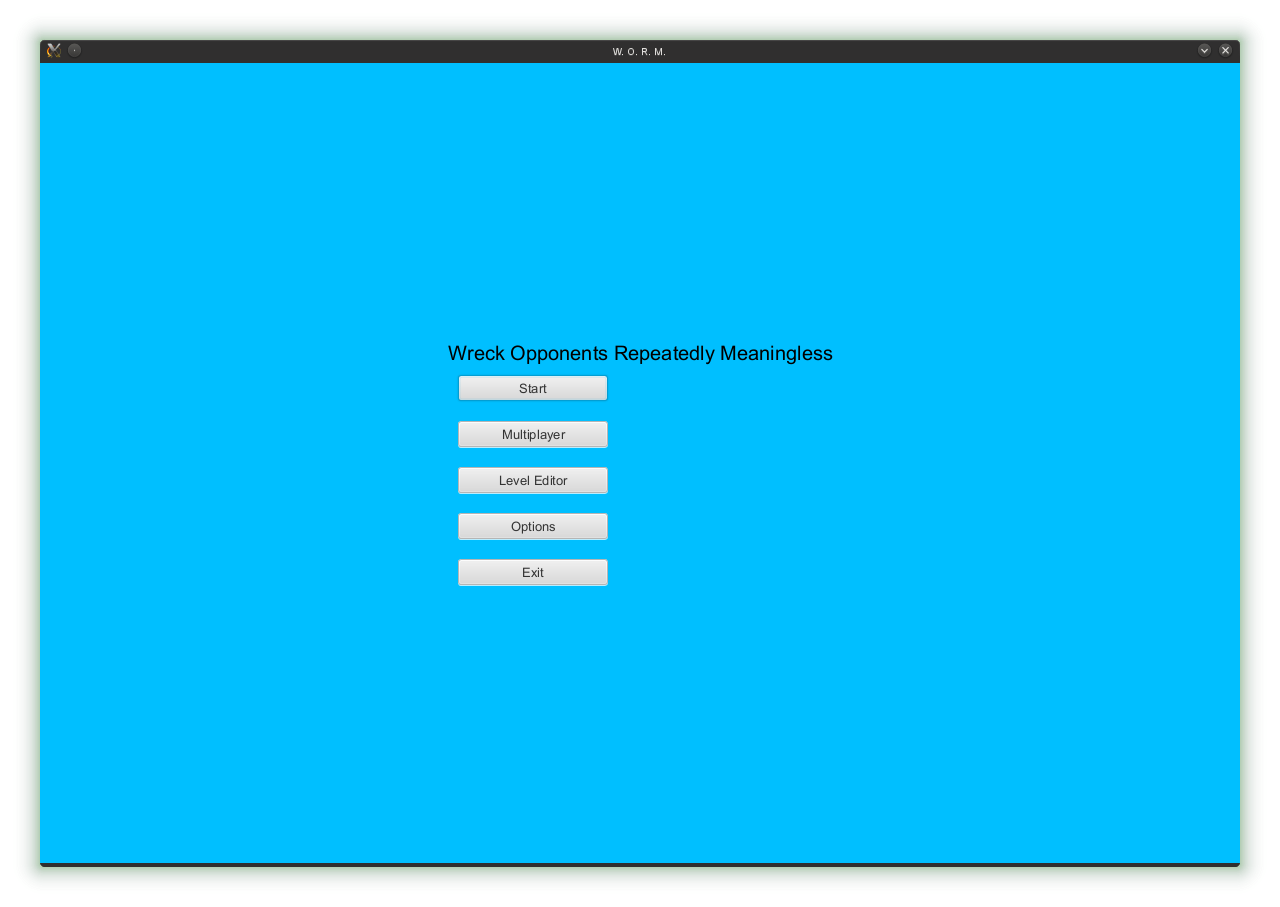
\includegraphics[height=9cm]{Screenshot1.png}

Start – Siehe Kapitel Das Spiel

Multiplayer – Siehe Kapitel Multiplayer

Level Editor – Siehe Kapitel Level Editor

Options – Siehe Kapitel Optionen

Exit – Schließt das Spiel

\chapter{Das Spiel}

\section{Ein Spiel erstellen}

Durch das Klicken auf den Start-Knopf im Hauptmenü gelangen wir zu den Spielereinstellungen.

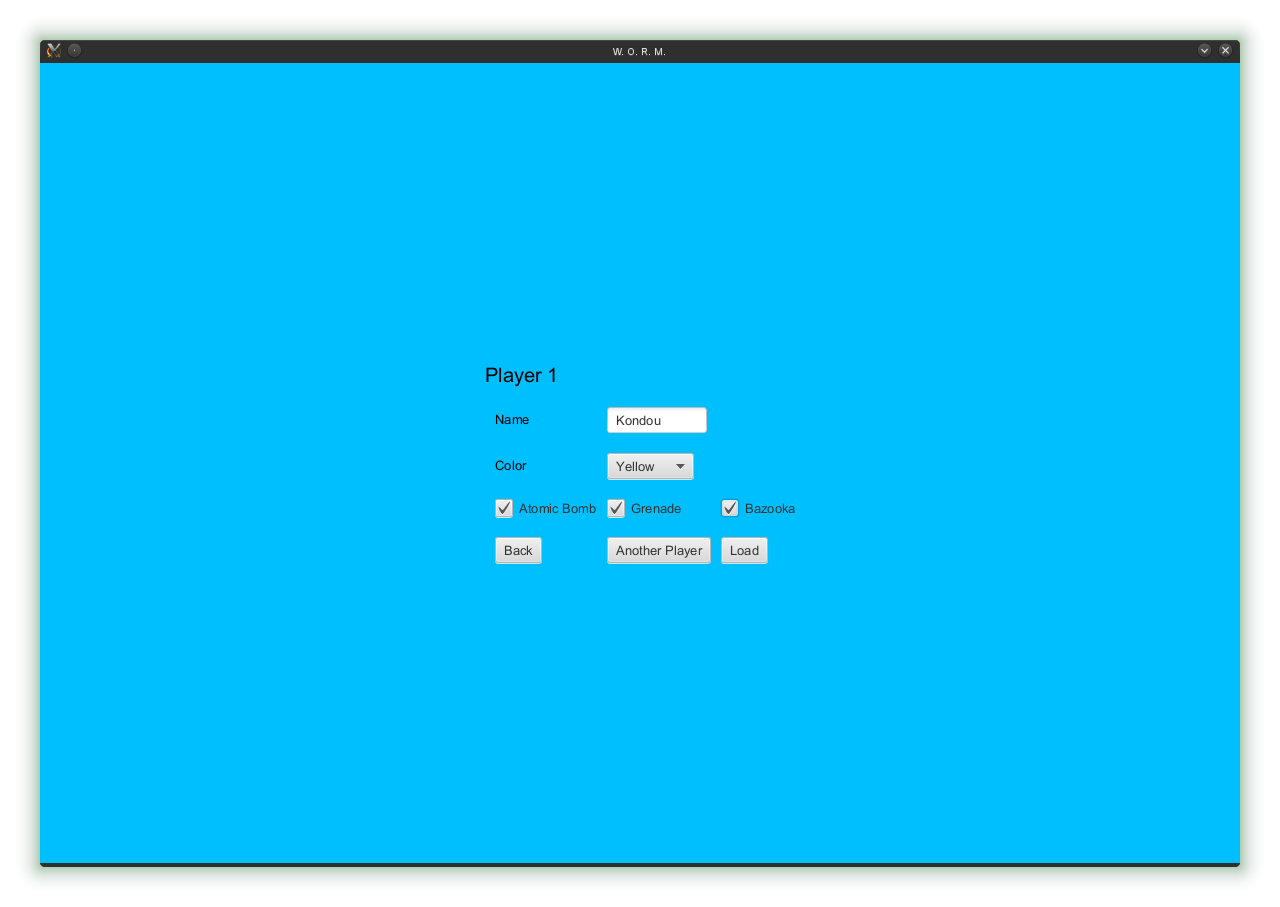
\includegraphics[height=9cm]{Screenshot5.png}

Jeder Spieler hat die Möglichkeit seinem Team einen Namen zu geben.
Neben Farbeinstellung ist es zudem wichtig mind. eine Waffe auszuwählen, da die Würmer sonst
nicht kämpfen können.

Alternativ lässt sich über den Load-Knopf auch ein bereits gespeichertes Spiel laden.

Nach der Einstellung des Ersten Spielers kann durch das Klicken auf den Knopf Another Player
der zweite Spieler seine Team erstellen.

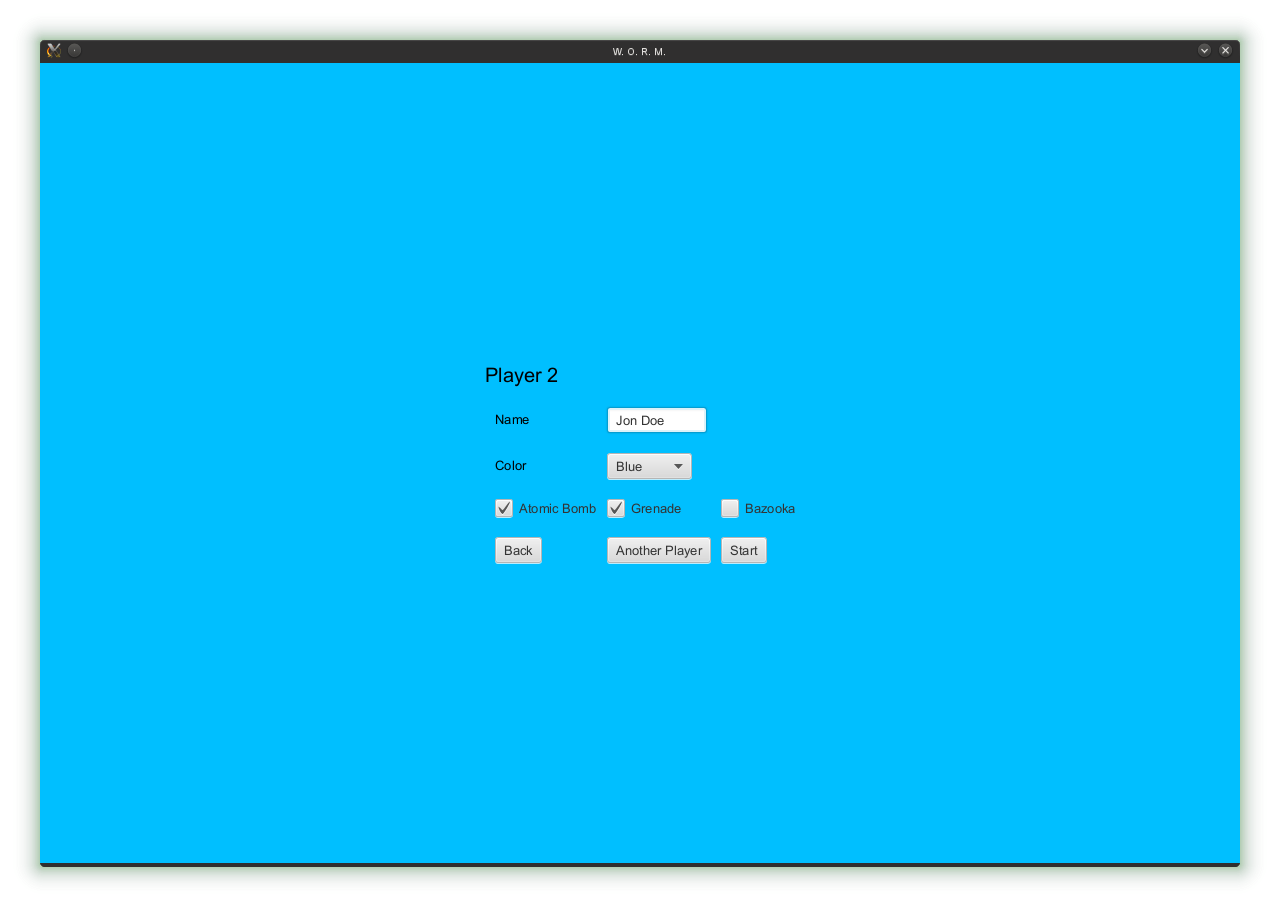
\includegraphics[height=9cm]{Screenshot6.png}

Durch den Back Knopf gelangt man wieder zurück zum Hauptmenü.

Nach der Teamerstellung des zweiten Spielers kann entweder noch ein dritter oder vierter Spieler
hinzugefügt werden, oder das Spiel gestartet werden.

Durch das Klicken auf den Start-Knopf gelangt man in die Leveleinstellung, wo die Mög\-lichkeit
besteht 8 vordefinierte Levelkarten zu wählen.

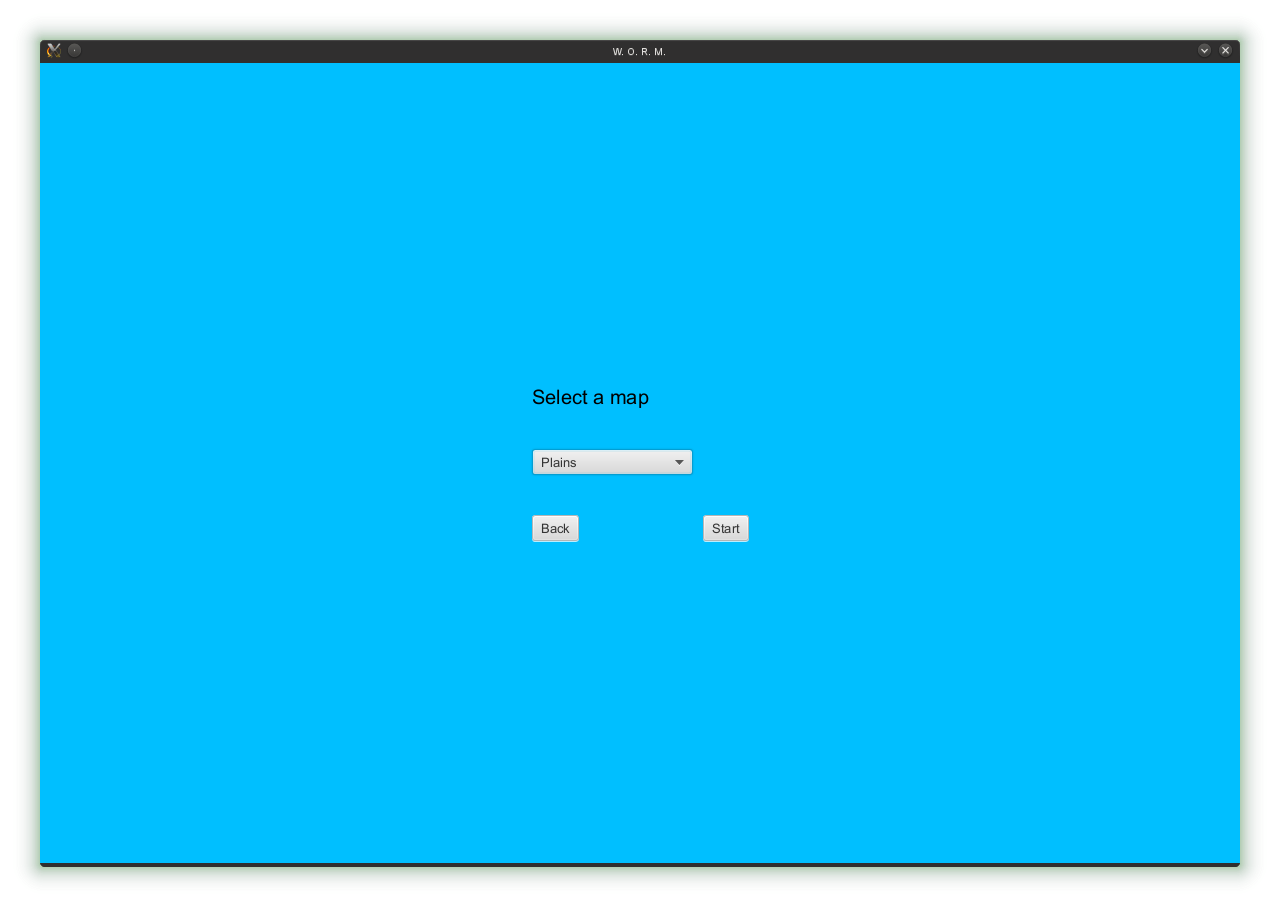
\includegraphics[height=9cm]{Screenshot7.png}

Die Levelkarte Random stellt dabie einen Spezialfall dar, da jene zufallsgeneriert Level erstellt.

Wenn wir jetzt auf Start drücken gelangen wir zur gewählten Levelkarte und beginnen das Spiel
mit dem Team von Spieler 1.

\section{Das Spiel}

\subsection{Erläuterung der Oberfläche}

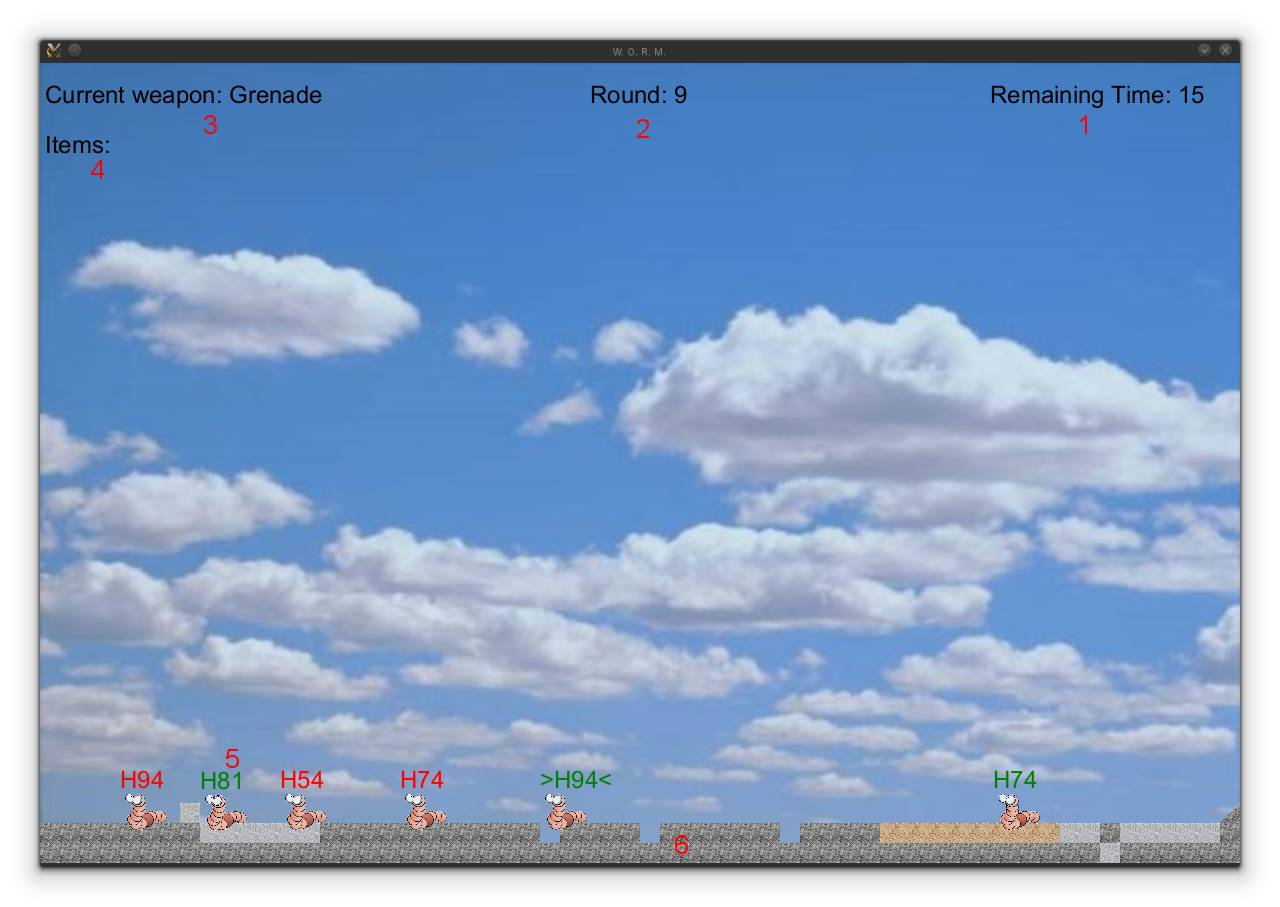
\includegraphics[height=9cm]{Screenshot13.jpg}

\begin{enumerate}
 \item Verbleinde Zeit für die Runde
 \item Rundennummer
 \item Ausgewählte Waffe
 \item Aufgesammelte Items des aktuellen Wurms
 \item Wum mit Lebenspunkten über seinem Kopf – der mit \texttt{><} eingerahmte Wurm ist zur Zeit am Zug
 \item Untergrund
\end{enumerate}

\subsection{Bedienung}

\subsubsection{Bewegung}

Durch die Tastaturpfeilknöpfe Rechts und Links bewegen sich die Würmer nach rechts oder links.

Durch den Tastaturknopf Oben können die Würmen in die vorher ausgewählte Richtung (Rechts oder Links) springen.

\subsubsection{Schießen}

Die Waffen die Sie vorher in den Teameinstellungen gewählt haben werden nun in der oberen linken Ecke des Fensters angezeigt.
Durch Scrollen mit dem Mausrad wechseln sie zwischen den Waffen.

Mit dem Mauszeiger zeigen sie den Waffen die Höhe und Weite des Schusses an. Dabei gibt die Richtung an, in welche Richtung
geschossen werden soll, und die Entfernung zum Wurm an, wie start geschossen werden soll.

Durch die rechte Maustaste können die Würmer ihre ausgewählte Waffe abschiessen.

\subsection{Item}

Es gibt 3 verschiedene Items. Jedes Item kann eingesammelt werden und werden dann oben links im Fenster angezeigt.
Die Items werden nummeriert und beim Drücken dieser Nummer verwendet. 

Elixir: Dieses Item verdoppelt das vorhandene Leben des Wurmes

Schuh: Durch dieses Item können die Würmer schneller auf Sand laufen.

Sprungfeder: Mit diesem Item können die Würmer noch höher springen.

\subsection{Lebenspunkte}

Jeder Wurm bekommt durch die Teameinstellung eine Farbe zugeordnet. Das Leben erscheint in der augewählten Farbe über jeden
Wurm. Jeder Wurm erhält zu Beginn des Spieles 100 Lebenspunkte.

Das Leben verringert sich dann, wenn ein Wurm von einem Geschoss getroffen wird oder, wenn er von einer großen Höhe fällt.

Ein Wurm ist dann Tod, wenn er kein Leben mehr hat oder außerhalb des Spielfeldes springt.

\chapter{Multiplayer}

Neben dem lokalen Mehrspieler-Modus ist auch ein online Spiel, über einen Internet Server möglich.

\section{Eigener Server}

Der Standardserver, schaepers.it ist für unkomplizierte online Spiele nutzbar, jedoch ist auch eine Einrichtung und Betrieb eines
eigenem Servers möglich.

Dafür startet man die beiliegende Server.jar Datei entweder direkt im Dateibrowser, oder in der Kommandozeile mit dem Kommando
\texttt{java -jar Server.jar}.

Zu beachten ist, dass, wer sich hinter einer NAT befindet den Port 7601 forwarden muss.

\section{Lobby}

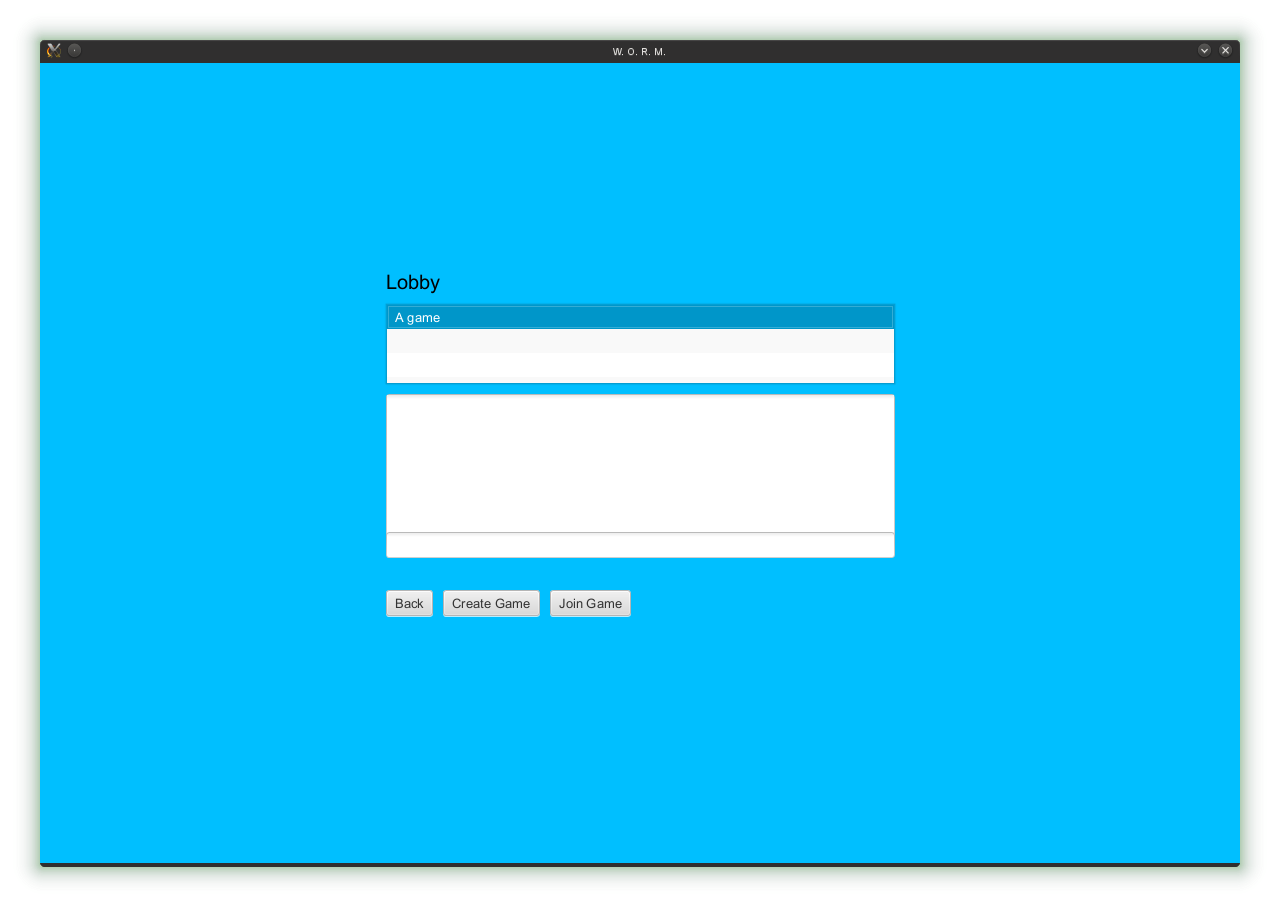
\includegraphics[height=9cm]{Screenshot8.png}

Dies ist der Lobby Bildschirm. Hier kann man entweder mit anderen Spielern auf dem gleichen Server global chatten, oder einem
Spiel beitreten.

Mit dem Back Knopf kommt man zurück ins Hauptmenü.

Mit dem Create Game Knopf kann man einen Raum erstellen, siehe dafür den Abschnitt Raum erstellen.

Mit dem Join Game Knopf können Sie dem oben ausgewähltem Spiel beitreten.

\section{Raum}

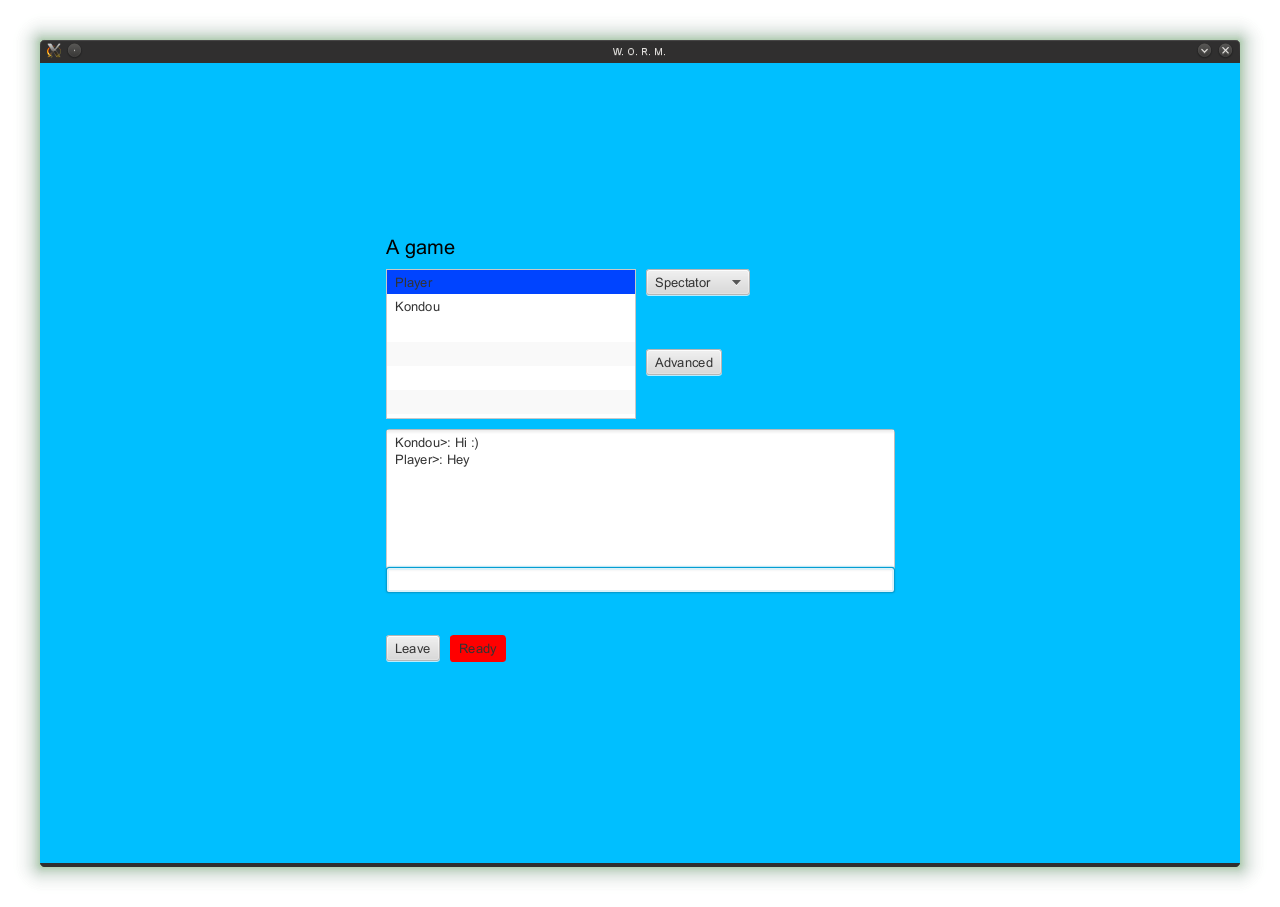
\includegraphics[height=9cm]{Screenshot10.png}

Dies ist der Raum Bildschirm, hier werden die Spieler in diesem Raum, mit ihren entsprechenden Team-Farben (oder weiß, für
Zuschauer) angezeigt. Außerdem besteht auch hier wieder die Möglichkeit mit den Spielern in diesem Raum zu chatten.

Mit dem Leave Knopf wird der jetzige Raum verlassen, und zum Lobby Bildschirm zurückgekehrt.

Mit dem Ready Knopf setzt sich der Spieler bereit um zu spielen, dabei gibt die Farbe den Status an. Grün steht für bereit,
Rot steht für nicht bereit.\\
Der Spiel-Leiter hat keinen Ready Knopf, sondern stattdessen einen Start-Knopf, welcher das Spiel startet. Die Farbe des Start
Knopfes zeigt hier an, ob alle Spieler bereit sind, indem er grün ist, oder nicht, indem er rot ist.

\subsection{Raum erstellen und bearbeiten}

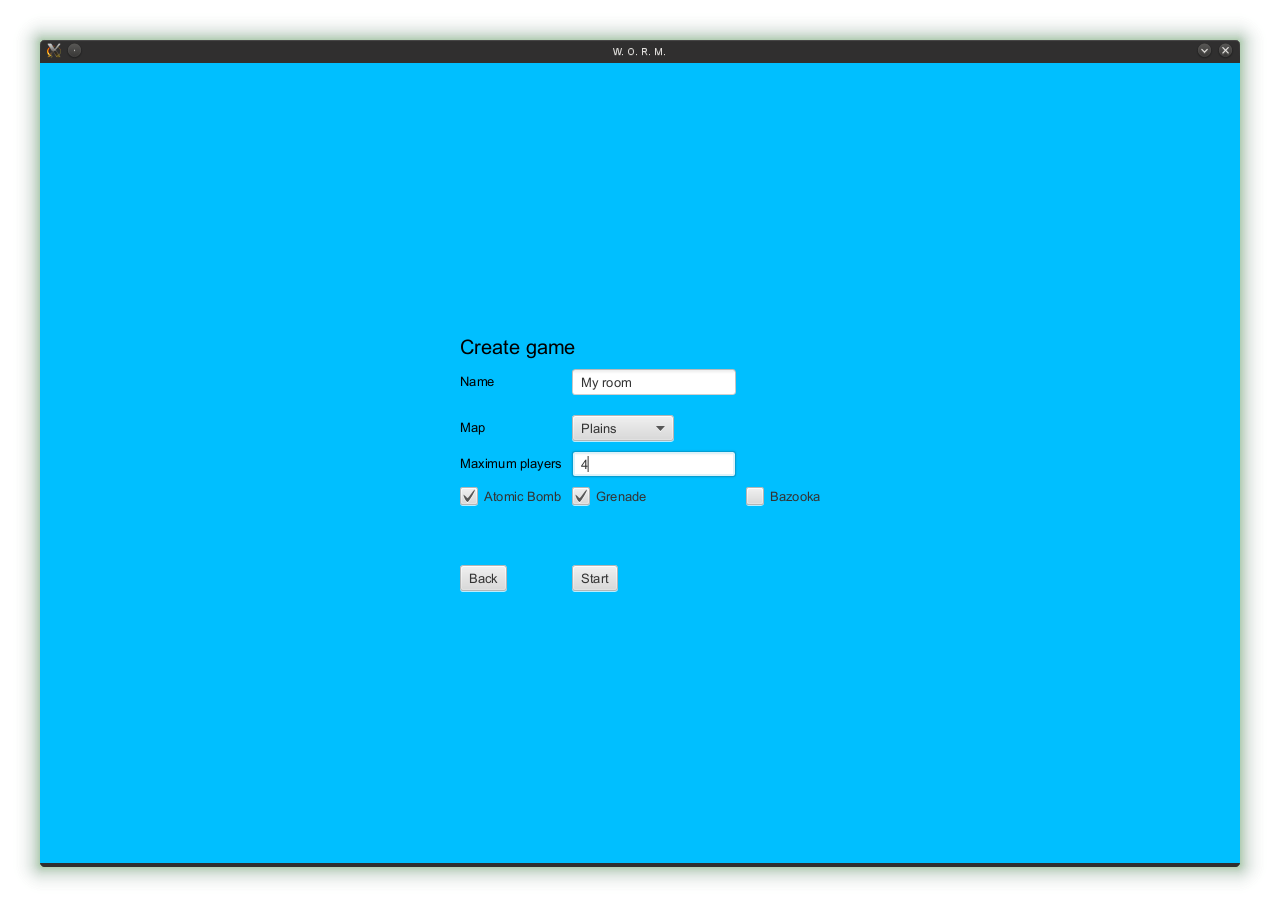
\includegraphics[height=9cm]{Screenshot14.png}

Mit dem Create Room Knopf aus dem Lobby Bildschirm lässt sich ein Raum erstellen.

Hier lässt sich nun der Name des Raumes einstellen, die Karte auf der gespielt werden soll, die maximale Anzahl an Spielern, die
in diesen Raum dürfen, und welche Waffen benutzt werden dürfen.

Der Back Knopf führt zurück zum Lobby-Bildschirm, der Start-Knopf erstellt den Raum.

Das Raum bearbeiten über den Advanced-Knopf im Raum-Bildschirm funktioniert analog, nur dass dann der Back-Knopf zurück zum Raum
führt, und der Change Properties-Knopf die Änderungen übernimmt.

\section{Multiplayer Spiel}

Das Multiplayer Spiel funtioniert ähnlich wie das Einzelspieler Spiel, nur, dass eine Person nur ein Team an Würmern kontrollieren
kann, und auf den Zug der anderen Person warten muss, für den Fall, dass sie zur Zeit nicht am Zug ist.

\subsection{Chat}

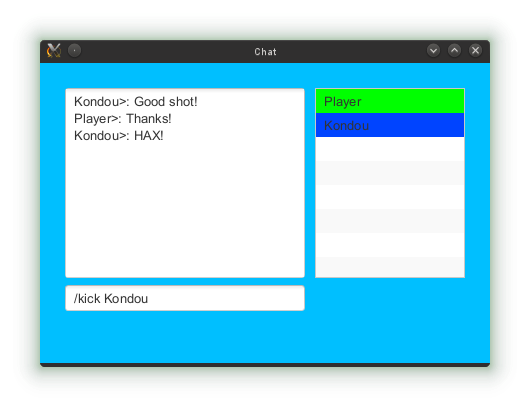
\includegraphics[height=9cm]{Screenshot12.png}

Ein weiteres Feature im Mehrspieler Spiel ist der Chat, dort lässt sich auch während des Spiels chatten.

Der Spielleiter kann außerdem Spieler aus dem Spiel werfen, in dem er \texttt{/kick [Spielername]} schreibt, und mit Enter
abschickt.

\chapter{Level Editor}

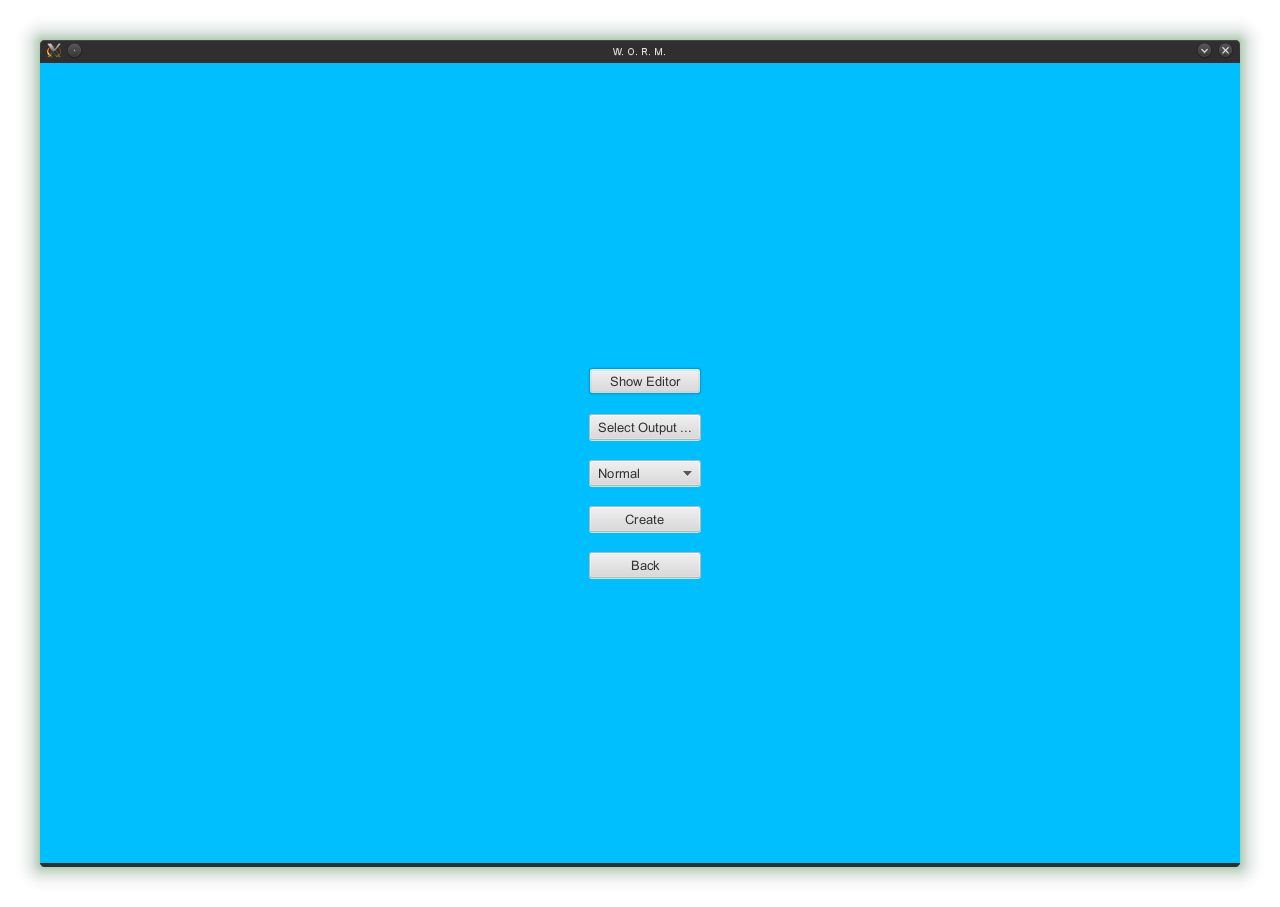
\includegraphics[height=9cm]{Screenshot3.png}

Im Hauptmenü wird durch das Drücken auf den \underline{Level Editor} Knopfs ein Fenster geöffnet mit der Möglichkeit ein Level selber zu erstellen.

Der Button \underline{Show Editor} zeigt das Level, das bearbeitet werden kann. Dort kann man durch mehreres Klicken der linken
Maustaste die verschieden Böden oder Items auswählen. Durch die rechte Maustaste kann man die Wurmpositionen festlegen.

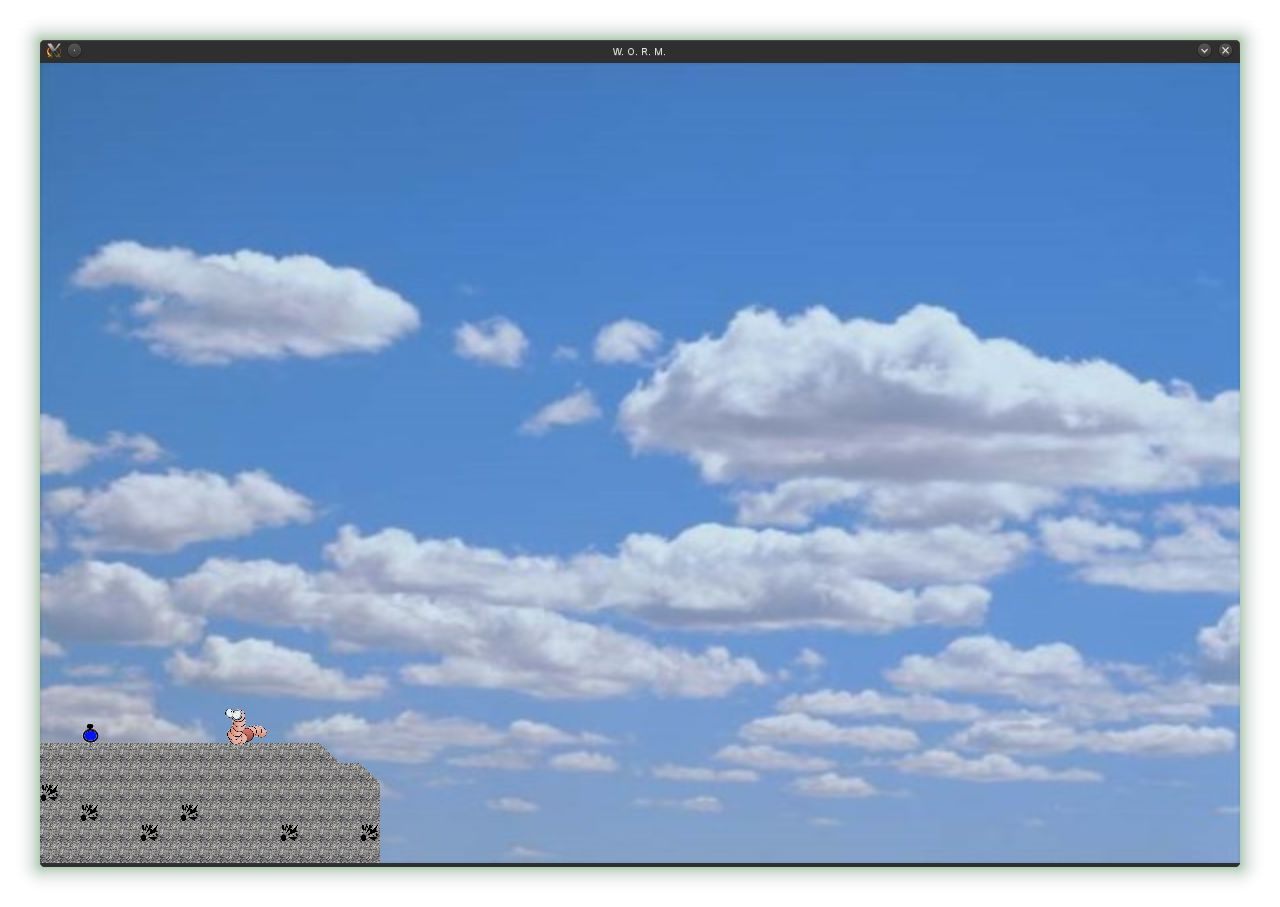
\includegraphics[height=9cm]{Screenshot4.jpg}

\underline{Select Output…} Bei klick öffnet sich ein Fenster, bei dem ausgewählt werden kann, wo genau das erstellte Level
gespeichert werden soll. Dies ist nötig, um das Level zu speichern. Jene Karten sollten neben der W.O.R.M.jar in einem eigens
erstellten Verzeichnis \texttt{maps} gespeichert werden, da Karten in diesem Verzeichnis vom Programm erkannt werden und bei der
Einzelspieler Kartenauswahl zur Verfügung stehen.

Der 3 Knopf lässt sie verschiedene Themen und Hintergründe auswählen, mit denen sie dann die Möglichkeit haben im normalem, horror oder orientalischem Stil ihr Level und den Hintergrund zu gestalten.

Durch das Drücken des \underline{Create} Knopfs erstellen sie den Level unter angegebenem Pfad.

Mit dem Knopf \underline{Back} gelangen Sie wieder ins Hauptmenü.

\chapter{Optionen}
Wenn wir nun auf Optionen klicken, erhalten wir ein Fenster mit verschiedenen Einstellungen.

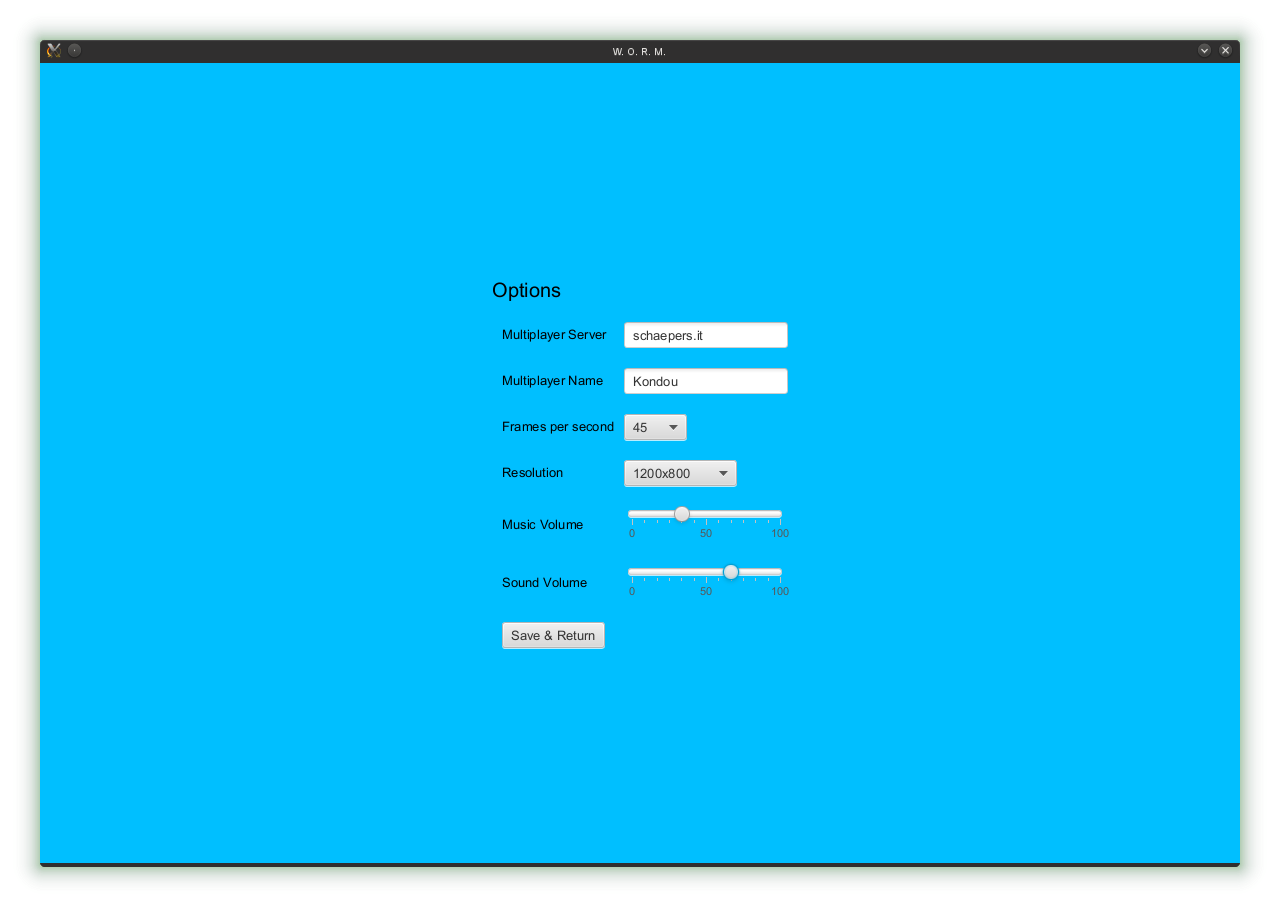
\includegraphics[height=9cm]{Screenshot2.png}

\underline{Multiplayer Server}\\
Hier lässt sich einstellen, mit welchem Server sich für online Spiele verbunden werden soll. Der standard Server ist hierbei von
Christopher Schäpers angeboten unter der Domain schaepers.it

\underline{Multiplayer Name}\\
Hier lässt sich der eigene Name für online Spiele einstellen. Diese Option empfiehlt sich sehr, da sonst jede Person den Namen
Worms-Player hat.

\underline{Resolution}\\
Dies stellt die Auflösung des Fensters ein. Erst nach speichern der Einstellungen wird jene angewandt.

\underline{Music-Volume}\\
Dieser Slider ändert die Lautstärke der Musik die Sie im Hintergrund hören. Dabei ziehen Sie den Slider nach links um
die Lautstärke zu verringern und nach rechts um sie zu erhöhen.

\underline{Sound-Volume}\\
Dieser Slider ändert, analog zu Music-Volume die Lautstärke der Geräuscheffekte die durch Abschießen der Waffen oder das Treffen
der Würmer ertönt.

Nach klick auf \underline{Save\&Return} werden die Einstellungen gespeichert, angewandt, und Sie gelangen zurück ins Hauptmenü.

\end{document}